% Название разделов -- все прописные
\section{ТЕОРЕТИЧЕСКАЯ ЧАСТЬ}
\subsection{Отделение неотложной медицинской помощи}
Отделение неотложной медицинской помощи является неотъемлемым и важнейшим структурным подразделением поликлиники или амбулаторно-поликлинического учреждения. Оно функционирует как специализированное подразделение, известное как отделение неотложной медицинской помощи, которое занимается оказанием немедленной и оперативной медицинской помощи лицам, столкнувшимся с внезапными острыми заболеваниями, состояниями или обострениями хронических недугов. Важно отметить, что помощь, оказываемая в этом отделении, специально предназначена для случаев, не представляющих угрозы для жизни и не требующих экстренной специализированной медицинской помощи.

Основная задача отдела неотложной медицинской помощи - оперативно и эффективно удовлетворять неотложные потребности пациентов в медицинской помощи, обеспечивая при этом их общее благополучие и безопасность. Это подразделение продуманно организовано в структуре поликлиники, которая служит комплексным медицинским учреждением, включающим в себя амбулаторные услуги, общую медицинскую помощь и центр врачей общей практики или семейной медицины.

Медицинская помощь, оказываемая в отделении неотложной помощи, направлена на немедленное и эффективное лечение внезапных кризисов здоровья, острых заболеваний или обострений хронических заболеваний, не представляющих угрозы для жизни. Эта специализированная помощь может оказываться различными способами, в зависимости от тяжести и срочности каждого случая. Парамедики, обученные первичной доврачебной медико-санитарной помощи, способны оказывать первичную медицинскую помощь на месте чрезвычайной ситуации, тем самым расширяя сферу деятельности отделения за пределы поликлиники. Кроме того, врачи поликлиники оснащены всем необходимым для оказания первичной медико-санитарной помощи в отделении неотложной помощи, обеспечивая комплексное и непрерывное обслуживание.

Благодаря размещению отделения неотложной медицинской помощи в структуре поликлиники пациенты имеют доступ к широкому кругу медицинских специалистов, учреждений и ресурсов, что в совокупности улучшает их медицинское обслуживание. Такая интеграция службы неотложной помощи в более широкое медицинское учреждение способствует созданию непрерывного процесса оказания помощи, гарантируя, что пациенты получат соответствующий уровень медицинской помощи, необходимый для эффективного решения их неотложных медицинских потребностей.
При изучении использовались ресурсы: \cite{11}, \cite{12},  \cite{13}.

\subsection{Электрокардиограмма}

Электрокардиограмма (ЭКГ) - это жизненно важный диагностический инструмент, используемый для исследования функции сердца, предлагающий неинвазивный и неспециализированный метод подготовки. С помощью ЭКГ кардиологи получают доступ к подробной и незаменимой информации о состоянии здоровья сердца пациента.

Эта диагностическая процедура имеет важное значение, поскольку позволяет получить ценные сведения о состоянии сердца пациента. Записывая электрическую активность сердца, ЭКГ позволяет кардиологам оценить различные аспекты сердечной деятельности, такие как частота сердечных сокращений, ритм, наличие каких-либо отклонений или нарушений. Эти данные имеют решающее значение для диагностики и мониторинга различных заболеваний, связанных с сердцем, что позволяет своевременно принимать необходимые меры для оптимизации лечения пациентов.

Неинвазивный характер ЭКГ делает ее привлекательной и доступной для пациентов, поскольку она не требует специальной подготовки или инвазивных процедур. Она включает в себя установку электродов на кожу пациента, которые улавливают и регистрируют электрические сигналы, генерируемые сердцем. Эта безболезненная процедура может быть выполнена быстро, что делает ее удобным и эффективным средством оценки сердечной функции.

Информация, полученная с помощью ЭКГ, является уникальной и незаменимой в области кардиологии. Она дает кардиологам полный обзор состояния сердца пациента, помогая выявить потенциальные отклонения, такие как аритмии, нарушения проводимости или ишемические изменения. Кроме того, ЭКГ служит в качестве исходного уровня для будущих сравнений, облегчая отслеживание состояния сердца пациента с течением времени.

В целом, электрокардиограмма служит фундаментальным и бесценным диагностическим инструментом в области кардиологии. Ее неинвазивный характер, простота использования и способность предоставлять подробную информацию о состоянии сердца пациента делают ее важным компонентом комплексной оценки состояния сердца. Используя возможности ЭКГ, кардиологи могут собирать важнейшие данные для диагностики, планирования лечения и постоянного мониторинга, что в конечном итоге повышает качество обслуживания и улучшает результаты лечения пациентов.
При изучении использовались ресурсы: \cite{21}, \cite{22}.

\subsection{Компьютерное зрение}

Компьютерное зрение - это междисциплинарная область, которая объединяет различные методы из информатики, математики и нейронауки, позволяющие компьютерам понимать и интерпретировать визуальную информацию. Она включает в себя разработку алгоритмов и моделей, которые могут анализировать и извлекать значимую информацию из цифровых изображений или видео.

Машинное обучение, в частности сверточные нейронные сети (CNN), сыграло значительную роль в продвижении задач компьютерного зрения. CNN - это тип модели глубокого обучения, специально разработанный для обработки данных, похожих на сетку, таких как изображения. Они состоят из нескольких слоев взаимосвязанных узлов, которые выполняют сверточные операции, позволяя сети изучать иерархические представления визуальных характеристик.

Задачи компьютерного зрения, в которых используются методы машинного обучения, включают:

\begin{itemize}
    \item Классификация изображений: Эта задача включает в себя присвоение метки или класса входному изображению, например, определение того, есть ли на изображении кошка или собака. CNN отлично справляются с классификацией изображений, обучаясь распознавать и различать различные визуальные модели,
    \item Обнаружение объектов: Обнаружение объектов направлено на поиск и классификацию нескольких объектов в кадре изображения или видео. Это включает в себя построение ограничительных рамок вокруг обнаруженных объектов и присвоение им соответствующих меток. Подходы на основе CNN, такие как популярные Faster R-CNN и YOLO (You Only Look Once), значительно расширили возможности обнаружения объектов,
    \item Сегментация изображения: Сегментация изображения подразумевает разделение изображения на значимые области или сегменты. Эта задача позволяет получить более точную информацию об объектах, присутствующих на изображении. Для сегментации изображений обычно используются CNN с архитектурами типа U-Net и Mask R-CNN,
    \item Обработка изображений: Методы компьютерного зрения также включают в себя различные задачи обработки изображений, такие как обесцвечивание, улучшение, восстановление и сверхразрешение. Для решения этих задач используются методы машинного обучения, включая CNN и генеративные состязательные сети (GAN).
\end{itemize}

Компьютерное зрение имеет широкий спектр применения, включая автономные транспортные средства, распознавание лиц, системы наблюдения, медицинскую визуализацию, дополненную реальность, робототехнику и многое другое. Достижения в области машинного обучения, особенно глубокого обучения, внесли большой вклад в прогресс и успех систем компьютерного зрения в последние годы.

Существуют дополнительные задачи и приложения, которые возникают благодаря распознаванию образов и компьютерному зрению. Давайте рассмотрим некоторые из них:

\begin{itemize}
    \item Поиск изображений по контексту: Поиск изображений по контексту подразумевает извлечение изображений из большого набора данных на основе определенных критериев или сходства. Это может быть сделано путем поиска изображений, похожих на целевое изображение, или с помощью текстовых описаний для поиска определенных атрибутов или объектов на изображениях. Эта задача требует применения таких методов, как поиск изображений на основе содержания, и может быть полезна в различных областях, таких как электронная коммерция, системы управления содержанием и базы данных изображений,
    \item Обнаружение положения: Определение положения включает в себя оценку положения, ориентации или позы объекта относительно камеры или опорной точки. Это очень важно в таких приложениях, как роботизированные манипуляции, дополненная реальность и автономная навигация. Алгоритмы компьютерного зрения могут анализировать визуальные данные и предоставлять информацию о положении объекта, обеспечивая точное управление и взаимодействие с окружающей средой,
    \item Оптическое распознавание символов: OCR - это технология, которая распознает и извлекает текст из изображений или отсканированных документов. Она включает в себя идентификацию отдельных символов или областей текста и преобразование их в машиночитаемые и редактируемые форматы. OCR находит применение в оцифровке печатных документов, автоматизированном вводе данных, индексировании документов и преобразовании текста в речь,
    \item Распознавание лиц: Распознавание лиц - это популярная задача компьютерного зрения, которая включает в себя идентификацию или проверку людей на основе их черт лица. В ней используются алгоритмы для обнаружения и анализа лицевых ориентиров, узоров и уникальных характеристик. Распознавание лиц имеет различные применения, включая системы проверки личности, системы наблюдения, контроль доступа и маркировку в социальных сетях,
    \item Распознавание формы: Распознавание формы включает в себя понимание и интерпретацию форм или рисунков, сделанных людьми. Они могут варьироваться от простых геометрических фигур до более сложных объектов. Эта задача требует алгоритмов, которые могут анализировать и классифицировать визуальные модели на основе их форм. Распознавание форм находит применение в распознавании эскизов, цифровом искусстве, интерпретации диаграмм и автоматизированном проектировании.
\end{itemize}

Эти дополнительные задачи расширяют возможности и сферы применения компьютерного зрения, демонстрируя его широкое влияние в различных областях и отраслях. При изучении использовались ресурсы: \cite{31}, \cite{36}, \cite{32}, \cite{55}.

\subsection{Обработка изображений}

Обработка изображений особенно актуальна по нескольким причинам. 

Во-первых, задачи компьютерного зрения часто требуют огромных объемов данных. Обучение моделей такого объема может быть чрезвычайно ресурсоемким и дорогостоящим. Для решения этой проблемы такие компании, как OpenAI, часто публикуют архитектуры своих моделей и параметры обучения в открытом доступе, позволяя другим использовать предварительно обученные модели. Однако тонкая настройка этих моделей с помощью трансфертного обучения, которое предполагает их адаптацию для конкретных случаев использования, в значительной степени зависит от методов обработки изображений. Именно благодаря обработке изображений реальные приложения могут по-настоящему процветать и развиваться.

Изображения также могут сбивать с толку даже человеческий глаз. Показано на рисунке~\ref{fig:fig01}. 
\begin{figure}
  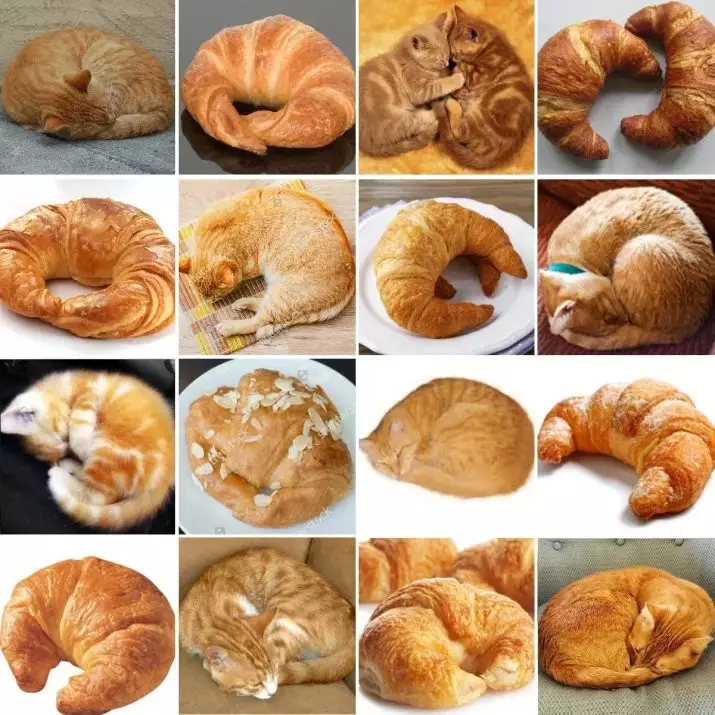
\includegraphics[scale=0.6]{inc/cat}
  \caption{Это кошка или круассан?}
  \label{fig:fig01}
\end{figure}


Способность тщательно обрабатывать, стандартизировать и дополнять изображения с помощью различных методов обработки играет решающую роль в повышении реалистичности и автоматизации сложных задач. Применяя обработку изображений, проблемы, связанные с этими сложными задачами, становятся более решаемыми, что облегчает автоматизированный анализ и интерпретацию.

Наконец, необходимо признать, что модели CV неизменно требуют ввода данных в виде изображений. Фактически, для приложений, основанных на видео, используются последовательности изображений. Это подчеркивает центральную роль изображений как основы для задач компьютерного зрения, подчеркивая важность методов обработки изображений для извлечения значимой информации и понимания из визуальных данных.

Таким образом, обработка изображений играет ключевую роль в компьютерном зрении, обеспечивая эффективную обработку данных, повышая адаптивность моделей и служа шлюзом для извлечения ценных знаний из визуальных данных.

Обработка изображений - это ряд операций, направленных на улучшение качества изображений для задач компьютерного зрения, чтобы они могли быть более предсказуемыми. 

Когда целью этих операций является увеличение количества доступных изображений, это обычно называют расширением изображений или данных. Это подразумевает создание дополнительных вариаций существующих изображений с помощью таких методов, как вращение, масштабирование, переворачивание, обрезка или введение случайного шума.

Важно отметить различие между предварительной обработкой изображений и дополнением данных. Предварительная обработка изображений применяется как на этапе обучения, так и во время вывода, обеспечивая надлежащую подготовку изображений к анализу. С другой стороны, увеличение данных применяется исключительно на этапе обучения, происходит после предварительной обработки изображений и служит для расширения разнообразия и надежности набора данных для обучения.

Входные данные для этих процессов обычно состоят из векторов признаков, представляющих интенсивность необработанных пикселей изображения. Эти векторы организованы в формате H x W x C, где H обозначает высоту изображения в пикселях, W - ширину в пикселях, а C - количество цветовых каналов, таких как красный, зеленый и синий (RGB).

Используя методы обработки изображений, исследователи и практики могут уточнять и оптимизировать визуальные данные, используемые в задачах компьютерного зрения, что в конечном итоге повышает точность, надежность и обобщающую способность соответствующих моделей.

Методы обработки изображений играют решающую роль в корректировке значений пикселей и формы изображений для создания стабильной математической основы для моделей. Некоторые выдающиеся методы в этой области включают:

\begin{itemize}
\item Нормализация: Эта техника включает преобразование значений пикселей в диапазон от 0 до 1. Нормализация особенно полезна, когда данные не соответствуют гауссовскому распределению. Путем изменения масштаба значений пикселей нормализация обеспечивает согласованное представление данных на различных изображениях,
\item Центрирование и стандартизация: Методы центрирования и стандартизации направлены на установление нулевого среднего значения для значений пикселей. Центрирование по изображениям корректирует каждое изображение отдельно, а центрирование по набору данных вычисляет среднее значение по всему набору данных. Стандартизация, в дополнение к центрированию, также направлена на достижение единичной дисперсии. Эти методы полезны, когда данные имеют гауссовское распределение. Рекомендуется поэкспериментировать с обоими подходами и выбрать тот, который обеспечивает наилучшую производительность для данной задачи,
\item Изменение размера: Изменение размера используется для изменения формы изображений, делая их однородными по размеру или масштабируя их с сохранением соотношения сторон. Эта техника гарантирует, что все изображения имеют одинаковые размеры или подвергаются последовательной корректировке размеров. Изменение размера упрощает обработку данных и позволяет моделям эффективно обрабатывать изображения,
\item Преобразование цветового канала: Преобразование цветовых каналов направлено на изменение количества цветовых каналов в изображении. Обычно оно включает преобразование изображений в формат градаций серого (1 канал), RGB (3 канала) или RGBA (4 канала), где RGBA включает альфа-канал, обозначающий непрозрачность. Эта техника обеспечивает совместимость с моделями, требующими определенных конфигураций цветовых каналов, а также может упростить вычисления и снизить сложность в определенных сценариях.
\end{itemize}

Благодаря применению этих методов обработки изображений данные, предоставляемые моделям компьютерного зрения, становятся более стандартизированными, что позволяет повысить производительность модели, улучшить обобщение и эффективно анализировать визуальную информацию.

Техники дополнения изображений гораздо более многочисленны, и лучший способ понять применяемые ими преобразования - визуальный, так что продеманстрируем это на рисунке~\ref{fig:fig02}.

\begin{figure}
  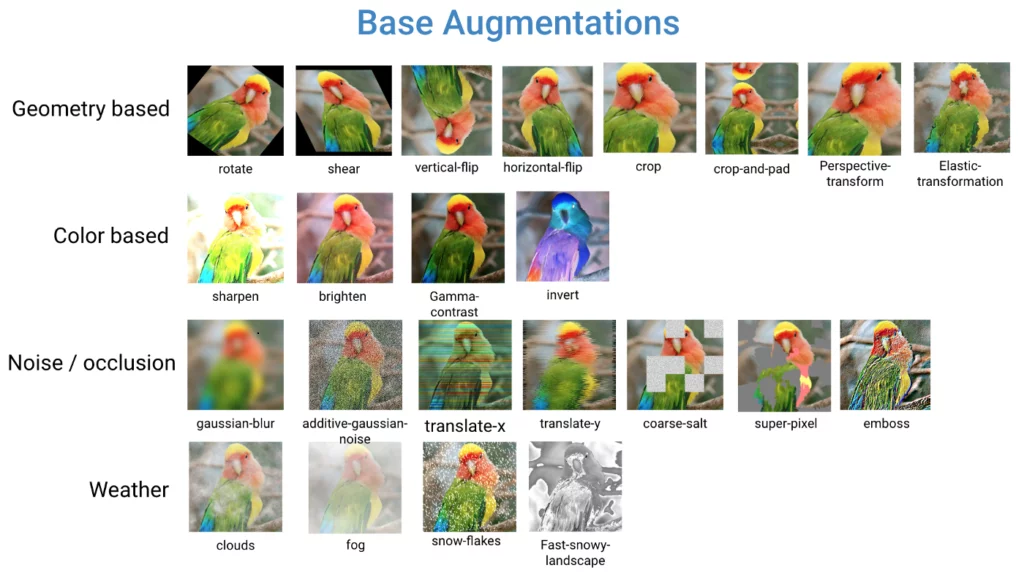
\includegraphics[scale=0.6]{inc/base}
  \caption{Визуальный обзор методов увеличения данных}
  \label{fig:fig02}
\end{figure}

Сфера фреймворков для обработки изображений в области машинного обучения обширна и предлагает множество вариантов. Выбор наиболее подходящего фреймворка часто может оказаться сложной задачей из-за обилия вариантов. Здесь я представляю список десяти наиболее часто используемых фреймворков обработки изображений для машинного обучения:


\begin{itemize}
    \item Pgmagick --- библиотека Python, взаимодействующая с программным обеспечением GraphicsMagick, предоставляющая возможности и функции обработки изображений,
    \item SimpleCV --- среда Python, разработанная для задач компьютерного зрения, включающая функции обработки и анализа изображений,
    \item TorchVision --- Часть экосистемы PyTorch, TorchVision предоставляет набор утилит для компьютерного зрения, включая функции обработки изображений,
    \item OpenCV --- чрезвычайно популярная библиотека компьютерного зрения с открытым исходным кодом, которая предлагает широкие возможности обработки изображений и доступна на нескольких языках программирования,
    \item Matlab --- собственная среда программирования, предоставляющая комплексные инструменты для обработки изображений, включая передовые алгоритмы и рабочие процессы,
    \item SciPy --- библиотека научных вычислений для Python, включающая различные модули, такие как scipy.ndimage, который предлагает функции обработки изображений,
    \item scikit-image --- библиотека Python, специально ориентированная на задачи обработки изображений, предоставляющая широкий спектр функций и алгоритмов,
    \item TensorFlow --- широко распространенная система глубокого обучения, которая также включает утилиты для обработки изображений, особенно с помощью модуля TensorFlow Image,
    \item Pillow/PIL --- библиотека Python Imaging Library (PIL) и ее дружественный форк Pillow предоставляют возможности обработки изображений, включая базовые операции, фильтрацию и преобразование форматов,
    \item NVIDIA OpenVINO --- набор инструментов с открытым исходным кодом от NVIDIA, который оптимизирует и ускоряет модели глубокого обучения, включая задачи обработки изображений, особенно для развертывания на оборудовании NVIDIA.
\end{itemize}

В то время как для специализированных задач машинного обучения может потребоваться использование сторонних или собственных фреймворков, в большинстве приложений компьютерного зрения для задач обработки изображений используются фреймворки с открытым исходным кодом.

Каждый из этих фреймворков предлагает стандартные методы обработки и дополнения изображений, зачастую незначительно различаясь в математической реализации. Несмотря на эти незначительные различия, фундаментальные концепции и функциональные возможности остаются неизменными.

Чтобы проиллюстрировать это, рассмотрим конкретный пример ~\ref{src:src1} ~\ref{src:src2}. преобразования изображения в градации серого, переворачивания его по горизонтали и обрезки по центру с помощью OpenCV и TensorFlow.

\begin{figure}
\begin{lstlisting}[language=Python]
import cv2 as cv

img = cv.imread('example.jpeg')

gray_img = cv.cvtColor(img, cv.COLOR_RGB2GRAY)

flipped_img = cv.flip(img, 0)

def crop_img(img, scale=1.0):
    center_x, center_y = img.shape[1] / 2, img.shape[0] / 2
    width_scaled, height_scaled = img.shape[1] * scale, img.shape[0] * scale
    left_x, right_x = center_x - width_scaled / 2, center_x + width_scaled / 2
    top_y, bottom_y = center_y - height_scaled / 2, center_y + height_scaled / 2
    img_cropped = img[int(top_y):int(bottom_y), int(left_x):int(right_x)]
    return img_cropped

cropped_img = crop_img(img, 0.7)
\end{lstlisting}
\caption{OpenCV}
\label{src:src1}
\end{figure} 


\begin{figure}
\begin{lstlisting}[language=Python]
import tensorflow as tf

img = tf.io.decode_jpeg(
    tf.io.read_file('example.jpeg'),
    channels=3,
)

gray_img = tf.image.rgb_to_grayscale(img)

flipped_img = tf.image.flip_up_down(img)

cropped_img = tf.image.central_crop(img, 0.7)
\end{lstlisting}
\caption{TensorFlow}
\label{src:src2}
\end{figure}

Если посмотреть на результат применения этих преобразований к изображению примера на рисунке ~\ref{fig:fig03}, то можно ожидать, что оба решения дадут одинаковый результат:

\begin{figure}
  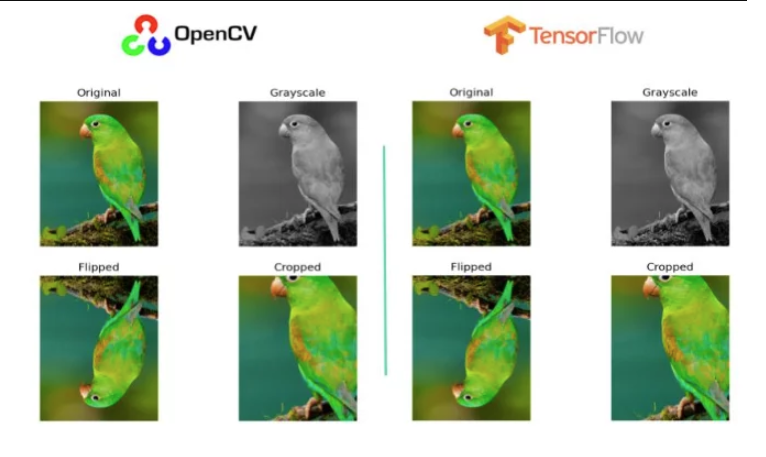
\includegraphics[scale=0.6]{inc/OpenCVTensorFlow}
  \caption{Преобразование изображений с помощью OpenCV (слева) и TensorFlow (справа)}
  \label{fig:fig03}
\end{figure}

Как вы можете видеть, код для выполнения этих операций с помощью OpenCV и TensorFlow довольно похож и дает эквивалентные результаты. Это показывает, что широко используемые фреймворки, как правило, обеспечивают последовательную реализацию стандартных методов обработки изображений, что позволяет относительно легко переключаться между фреймворками или выбирать тот, который лучше всего соответствует требованиям проекта.

В целом, этот пример подчеркивает совместимость и взаимозаменяемость популярных фреймворков для обработки изображений, укрепляя идею о том, что эти фреймворки предлагают стандартные методы с сопоставимыми результатами, обеспечивая пользователям гибкость и простоту использования.
При изучении использовались ресурсы: \cite{33}, \cite{35}, \cite{34}.

\subsection{Нормализация изображений}

Нормализация изображений - это важный этап предварительной обработки при подготовке наборов данных для задач искусственного интеллекта (ИИ), особенно в компьютерном зрении. Она включает в себя преобразование нескольких изображений в общее статистическое распределение по размерам и значениям пикселей. Кроме того, нормализация может применяться и к одному изображению для устранения неоднородностей или артефактов.

Пространственная нормализация направлена на выравнивание изображений с точки зрения их пространственного соотношения или положения. Она гарантирует, что соответствующие области интереса (ROIs) на разных изображениях имеют одинаковый размер, ориентацию или положение, что позволяет проводить справедливые сравнения. Этот процесс может включать масштабирование, поворот, перевод или даже нелинейные деформации для правильного выравнивания изображений. Регистрация изображений - это распространенная техника, используемая для достижения пространственной нормализации путем выравнивания изображений по определенным признакам или ориентирам.

Нормализация интенсивности, с другой стороны, направлена на нормализацию значений пикселей на всех изображениях или в пределах одного изображения. Она гарантирует, что общее распределение интенсивности пикселей будет одинаковым, что облегчает сравнение и анализ изображений. Нормализация значений интенсивности позволяет минимизировать вариации яркости, контраста и других характеристик изображения. Это особенно актуально для медицинской визуализации, например, МРТ, где артефакты поля смещения могут вызывать неоднородность интенсивности. Нормализация смещения сканирования, разновидность нормализации интенсивности, может применяться для устранения таких артефактов и достижения более равномерного распределения интенсивности по изображению.

В целом, нормализация изображения, охватывающая как пространственные аспекты, так и аспекты интенсивности, является важным этапом предварительной обработки в различных задачах компьютерного зрения. Она помогает стандартизировать и выровнять изображения, делая их более удобными для анализа, выделения признаков и последующих алгоритмов машинного обучения.

Распространенные методы нормализации:
\begin{itemize}
    \item Минимально-максимальное масштабирование позволяет изменить масштаб значений пикселей изображения до определенного диапазона, обычно от 0 до 1. Он предполагает нахождение минимального и максимального значений пикселей в изображении и линейное приведение этих значений к нужному диапазону. Min-max масштабирование полезно для обеспечения того, чтобы значения пикселей находились в стандартном диапазоне,
    \item Нормализация Z-score (также известная как стандартизация) преобразует значения пикселейтак, чтобы они имели нулевое среднее значение и единичную дисперсию. Она включает в себя вычитание среднего значения изображения и деление на стандартное отклонение. Нормализация Z-score эффективна при работе с изображениями с разными средними и стандартными отклонениями, приводя их к единой шкале,
    \item Выравнивание гистограммы - это метод, который повышает контрастность изображения путем перераспределения значений пикселей по спектру интенсивности. Она направлена на достижение более сбалансированной гистограммы, что приводит к улучшению качества изображения. Выравнивание гистограммы может быть особенно полезно для улучшения изображений с низким контрастом,
    \item Локальная нормализация контраста (например, адаптивная гистограммная эквализация, или AHE) - это метод, который повышает контраст в локализованных областях изображения. В отличие от глобальной гистограммной эквализации, она адаптирует процесс эквализации к меньшим регионам, сохраняя тем самым локальные детали. Локальная нормализация контраста может быть эффективна при улучшении изображений с различной освещенностью или контрастом в разных регионах.
\end{itemize}


Выводы по разделу

Представлены темы, в которых велись исследования для реализации проекта.
